\documentclass[aspectratio=169]{beamer}
\usetheme{boxes}
\usepackage{bm}
\usepackage{booktabs}
\usepackage{amsfonts}
\usepackage{amssymb}
\usepackage{amsmath}
\usepackage{amsthm}
\usepackage{comment}
\usepackage{geometry}
% Removed algorithmic packages to avoid conflicts
\usepackage{graphicx}
\usepackage{subcaption}
\usepackage{tikz}
% \usepackage{physics} % Removed due to conflicts with essay-def
\usepackage{xcolor}
\usepackage{listings}
\usepackage{essay-def}
% Configure itemize for beamer
\newcommand{\JX}[1]{{\color{blue}{$^{\text{JX}}$[#1]}}}
\setbeamertemplate{itemize item}{$\circ$}
\setbeamertemplate{itemize subitem}{\textbullet}
\usepackage[version=4]{mhchem}
\geometry{left=1cm,right=1cm}

% Define custom colors matching ByteDance style
\definecolor{highlight}{RGB}{220, 20, 60}
\definecolor{codegreen}{RGB}{0, 128, 0}
\definecolor{codepurple}{RGB}{128, 0, 128}

% Code listing style
\lstset{
  basicstyle=\ttfamily\footnotesize,
  keywordstyle=\color{blue},
  commentstyle=\color{codegreen},
  stringstyle=\color{codepurple},
  breaklines=true,
  frame=single,
  backgroundcolor=\color{gray!5}
}

\title[AI Agents]{AI Agents: From Tool Use to Intelligent Systems}
\subtitle{21 Days with Claude Code}
\author[J. Zhao \& CC]{Jiaxi Zhao (NUS) \& Claude Code (Anthropic)}
\date[\today]{\today}

\begin{document}

\begin{frame}
\titlepage
\end{frame}

\begin{frame}{Outline}
\tableofcontents
\end{frame}

% ==========================
% Section 1: What is Agent and Why Agent? (6 pages)
% ==========================
\section{What is Agent and Why Agent?}

\begin{frame}
	\begin{center}
		\Large
		\textbf{What is Agent and Why Agent?}
	\end{center}
\end{frame}

\begin{frame}{What is an Agent?}
	\begin{block}{Formal Definition (Russell \& Norvig)}
		"An agent is anything that perceives its \textbf{environment} through sensors and acts upon that environment through \textbf{actuators}."
	\end{block}
	
	\vspace{0.3cm}
	
	\begin{columns}
		\column{0.5\textwidth}
		\textbf{Key Characteristics:}
		\begin{itemize}
			\item {\color{highlight}\textbf{Autonomy}}: Acts independently
			\item {\color{highlight}\textbf{Perception}}: Senses environment
			\item {\color{highlight}\textbf{Action}}: Changes environment
			\item {\color{highlight}\textbf{Goal-directed}}: Works toward objectives
		\end{itemize}
		
		\column{0.5\textwidth}
		\textbf{In AI Context:}
		\begin{itemize}
			\item Software that performs tasks with minimal supervision
			\item Makes decisions to maximize goals
			\item Can learn and adapt over time
			\item Ranges from thermostats to LLMs
		\end{itemize}
	\end{columns}
	
	\vspace{0.3cm}
	
	\begin{center}
		\small
		{\color{gray}Etymology: From Latin \textit{agere} (to do) - "action on behalf of"}
	\end{center}
\end{frame}

\begin{frame}{Tool Use: Signal of Early Intelligence}
	\begin{columns}
		\column{\textwidth}
		\begin{itemize}
			\item {\color{highlight}\textbf{Anthropological perspective}}: Tool use marks cognitive revolution
			\begin{itemize}
				\item Stone tools $\rightarrow$ Agriculture $\rightarrow$ Writing systems
				\item Cognitive leap: from reactive to proactive behavior
			\end{itemize}
			\item {\color{highlight}\textbf{AI parallel}}: From language generation to action
			\begin{itemize}
				\item GPT-3 (2020): Pure text generation
				\item WebGPT (2021): Web browsing capability
				\item ChatGPT Plugins (2023): Third-party tool ecosystem
				\item Claude Code (2025): Full IDE integration
			\end{itemize}
		\end{itemize}
	\end{columns}
\end{frame}

\begin{frame}{Eliminating Hallucination Through Grounding}
	\begin{itemize}
		\item {\color{highlight}\textbf{Problem}}: LLMs generate plausible but incorrect information
		\item {\color{highlight}\textbf{Solution}}: Ground responses in external tools and data
	\end{itemize}
	
	\begin{columns}
		\column{0.5\textwidth}
		\begin{block}{Without Tools}
			\small
			\texttt{Q: What is sqrt(144)?} \\
			\texttt{A: sqrt(144) = 13} \\
			{\color{red}$\times$ Hallucination}
		\end{block}
		
		\column{0.5\textwidth}
		\begin{block}{With Calculator Tool}
			\small
			\texttt{Thought: Use calculator} \\
			\texttt{Action: calc(sqrt(144))} \\
			\texttt{Result: 12} \\
			\texttt{A: sqrt(144) = 12} \\
			{\color{green}$\checkmark$ Grounded}
		\end{block}
	\end{columns}
	
	\vspace{0.5cm}
	
	\begin{center}
		\textbf{Key Insight:} {\color{highlight}Grounding in external tools eliminates hallucination}
	\end{center}
\end{frame}

\begin{frame}{Environmental Interaction Paradigm}
	\begin{center}
		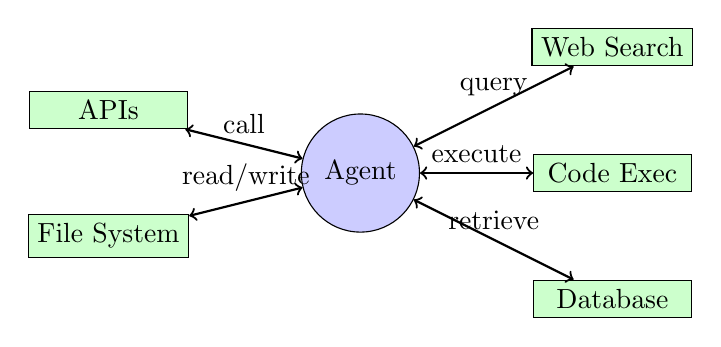
\begin{tikzpicture}[scale=0.8]
			% Agent
			\node[circle, draw, fill=blue!20, minimum size=1.5cm] (agent) at (0,0) {Agent};
			
			% Environment components
			\node[rectangle, draw, fill=green!20, minimum width=2cm] (web) at (4,2) {Web Search};
			\node[rectangle, draw, fill=green!20, minimum width=2cm] (code) at (4,0) {Code Exec};
			\node[rectangle, draw, fill=green!20, minimum width=2cm] (db) at (4,-2) {Database};
			\node[rectangle, draw, fill=green!20, minimum width=2cm] (api) at (-4,1) {APIs};
			\node[rectangle, draw, fill=green!20, minimum width=2cm] (file) at (-4,-1) {File System};
			
			% Arrows
			\draw[<->, thick] (agent) -- (web) node[midway, above] {query};
			\draw[<->, thick] (agent) -- (code) node[midway, above] {execute};
			\draw[<->, thick] (agent) -- (db) node[midway, above] {retrieve};
			\draw[<->, thick] (agent) -- (api) node[midway, above] {call};
			\draw[<->, thick] (agent) -- (file) node[midway, above] {read/write};
		\end{tikzpicture}
	\end{center}
	
	\begin{itemize}
		\item {\color{highlight}\textbf{Perception}}: Read from environment (search, query, read)
		\item {\color{highlight}\textbf{Action}}: Modify environment (write, execute, call)
		\item {\color{highlight}\textbf{Learning}}: Adapt based on feedback
	\end{itemize}
\end{frame}

% TEMP COMMENTED OUT FOR DEBUGGING
%\begin{frame}{Agent-Environment Interaction: RL Framework}
%	\begin{center}
%		\begin{tikzpicture}[scale=0.8]
%			% Agent
%			\node[rectangle, draw, fill=blue!30, minimum width=2.5cm, minimum height=1cm] (agent) at (0,0) {Agent (LLM)};
%			
%			% Environment
%			\node[rectangle, draw, fill=green!30, minimum width=3cm, minimum height=1.5cm] (env) at (6,0) {Environment\\Tools, APIs, Files};
%			
%			% State arrow
%			\draw[->, thick, red] (env) to[bend left=30] (agent) node[midway, above] {State $s_t$};
%			
%			% Action arrow  
%			\draw[->, thick, blue] (agent) to[bend left=30] (env) node[midway, below] {Action $a_t$};
%			
%			% Reward arrow
%			\draw[->, thick, purple] (env) to[bend left=60] (agent) node[midway, above left] {Reward $r_t$};
%		\end{tikzpicture}
%	\end{center}
%	
%	\vspace{0.3cm}
%	
%	\begin{columns}
%		\column{0.5\textwidth}
%		\textbf{RL Components:}
%		\begin{itemize}
%			\item {\color{red}State}: Context + tool outputs
%			\item {\color{blue}Action}: Tool calls + text generation  
%			\item {\color{purple}Reward}: Task success + human feedback
%		\end{itemize}
%		
%		\column{0.5\textwidth}
%		\textbf{Evolution via RL:}
%		\begin{itemize}
%			\item Learn which tools to use when
%			\item Improve reasoning strategies
%			\item Adapt to user preferences
%		\end{itemize}
%	\end{columns}
%	
%	\vspace{0.3cm}
%	\begin{center}
%		{\color{highlight}Agents can improve through environmental interaction}
%	\end{center}
%\end{frame}

\begin{frame}{Agent Learning Through Environment}
	\textbf{Key Concept:} Agents can evolve and improve through reinforcement learning
	
	\vspace{0.5cm}
	
	\begin{itemize}
		\item {\color{highlight}\textbf{State}}: Current context + tool outputs
		\item {\color{highlight}\textbf{Action}}: Tool calls + text generation
		\item {\color{highlight}\textbf{Reward}}: Task success + human feedback
	\end{itemize}
	
	\vspace{0.5cm}
	
	\textbf{Learning Goals:}
	\begin{itemize}
		\item Learn optimal tool selection
		\item Improve reasoning strategies  
		\item Adapt to user preferences
	\end{itemize}
\end{frame}

\begin{frame}{Evolution: From Prompting to Agents}
	\begin{center}
		\begin{tabular}{|l|c|c|c|c|}
			\hline
			\textbf{Capability} & \textbf{Prompting} & \textbf{Tool Use} & \textbf{Agents} & \textbf{Advanced} \\
			\hline
			User Control & High & Medium & Low & Guided \\
			Context Length & Limited & Limited & Extended & Extended* \\
			Error Recovery & Manual & Manual & Semi-auto & Semi-auto \\
			Task Complexity & Simple & Medium & Complex & Complex \\
			\hline
			\textbf{Example} & ChatGPT & Plugins & ReAct & Claude Code \\
			\hline
		\end{tabular}
	\end{center}
	
	\vspace{0.5cm}
	
	\begin{itemize}
		\item {\color{highlight}\textbf{Prompting Era}} (2020-2022): Chain-of-thought, few-shot learning
		\item {\color{highlight}\textbf{Tool Use Era}} (2022-2024): Function calling, structured outputs
		\item {\color{highlight}\textbf{Early Agent Era}} (2024-2025): Planning, memory, basic workflows
		\item {\color{highlight}\textbf{Future}} (2025+): Enhanced reliability, domain specialization
	\end{itemize}
	
\end{frame}

% ==========================
% Section 2: How to Build Agent? (5 pages)
% ==========================
\section{How to Build Agent?}

\begin{frame}
	\begin{center}
		\Large
		\textbf{How to Build Agent?}

	\end{center}
\end{frame}

\begin{frame}[fragile]{Tool Use Mechanism: From Text to Action}
	\begin{block}{Pattern Recognition for Tool Calls}
		LLMs output text $\rightarrow$ System recognizes patterns $\rightarrow$ Triggers tool execution
	\end{block}
	
	\begin{columns}
		\column{0.5\textwidth}
		\textbf{OpenAI Function Calling:}
		\begin{lstlisting}[basicstyle=\tiny]
{
  "role": "assistant",
  "content": null,
  "function_call": {
    "name": "get_weather",
    "arguments": "{\"location\": \"SF\"}"
  }
}
		\end{lstlisting}
		
		\column{0.5\textwidth}
		\textbf{ReAct Format:}
		\begin{lstlisting}[basicstyle=\tiny]
Thought: I need to search for weather in San Francisco
Action: Search[San Francisco weather]
Observation: Current weather in San Francisco is 72F, sunny
Thought: I now have the weather information needed
		\end{lstlisting}
	\end{columns}
	
	\vspace{0.3cm}
	\begin{itemize}
		\item {\color{highlight}\textbf{JSON Schema}}: Structured output for reliable parsing,
		Claude's tool use format
		\item {\color{highlight}\textbf{XML Tags}}: Better prompt readability and 
	\end{itemize}
\end{frame}

\begin{frame}[fragile]{MCP: Model Context Protocol}
	\begin{columns}
		\column{0.6\textwidth}
		\begin{itemize}
			\item {\color{highlight}\textbf{Standardized protocol}} for LLM-tool communication
			\item {\color{highlight}\textbf{Key Components}}:
			\begin{itemize}
				\item Resource discovery
				\item Tool registration
				\item Execution sandbox
				\item Result formatting
			\end{itemize}
			\item {\color{highlight}\textbf{Benefits}}:
			\begin{itemize}
				\item Tool interoperability
				\item Security isolation
				\item Consistent interfaces
			\end{itemize}
		\end{itemize}
		
		\column{0.4\textwidth}
		\begin{lstlisting}[language=python, basicstyle=\tiny]
# MCP Tool Definition
@mcp_tool
def search(query: str) -> str:
    """Search the web"""
    return web_api.search(query)

# Auto-registered with LLM
tools = discover_tools()
llm.register(tools)
		\end{lstlisting}
	\end{columns}
	
	\vspace{0.3cm}
	\begin{block}{MCP in Claude Code}
		Dynamically loads environment-specific tools at runtime, enabling IDE integration, file system access, and custom tool extensions
	\end{block}
\end{frame}

\begin{frame}{Agentic Workflows}
	\begin{center}
		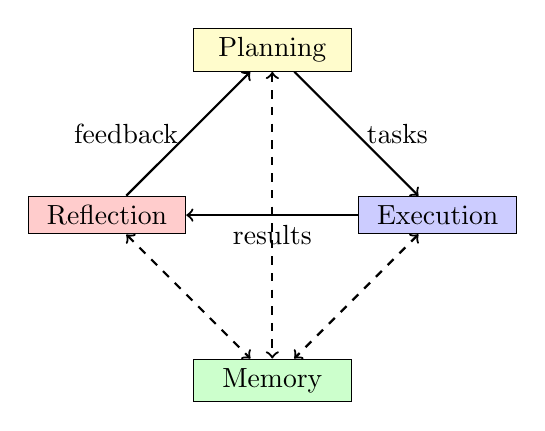
\begin{tikzpicture}[scale=0.7]
			% Planning
			\node[rectangle, draw, fill=yellow!20, minimum width=2cm] (plan) at (0,3) {Planning};
			
			% Execution
			\node[rectangle, draw, fill=blue!20, minimum width=2cm] (exec) at (3,0) {Execution};
			
			% Reflection
			\node[rectangle, draw, fill=red!20, minimum width=2cm] (reflect) at (-3,0) {Reflection};
			
			% Memory
			\node[rectangle, draw, fill=green!20, minimum width=2cm] (memory) at (0,-3) {Memory};
			
			% Arrows
			\draw[->, thick] (plan) -- (exec) node[midway, right] {tasks};
			\draw[->, thick] (exec) -- (reflect) node[midway, below] {results};
			\draw[->, thick] (reflect) -- (plan) node[midway, left] {feedback};
			
			\draw[<->, thick, dashed] (plan) -- (memory);
			\draw[<->, thick, dashed] (exec) -- (memory);
			\draw[<->, thick, dashed] (reflect) -- (memory);
		\end{tikzpicture}
	\end{center}
	
	\begin{columns}
		\column{0.5\textwidth}
		\begin{itemize}
			\item {\color{highlight}\textbf{Planning}}: Task decomposition
			\item {\color{highlight}\textbf{Execution}}: Tool calls, actions
		\end{itemize}
		
		\column{0.5\textwidth}
		\begin{itemize}
			\item {\color{highlight}\textbf{Reflection}}: Self-critique
			\item {\color{highlight}\textbf{Memory}}: Context persistence
		\end{itemize}
	\end{columns}
\end{frame}

\begin{frame}{Training Agents: Beyond Pre-training}
	\begin{tabular}{|l|p{3cm}|p{3cm}|p{3cm}|}
		\hline
		\textbf{Stage} & \textbf{Pre-training} & \textbf{Fine-tuning} & \textbf{Agent Training} \\
		\hline
		\textbf{Objective} & Next token prediction & Task-specific & Tool use + Planning \\
		\hline
		\textbf{Data} & Web text & Labeled examples & Trajectories \\
		\hline
		\textbf{Scale} & Trillions of tokens & Thousands & Millions of steps \\
		\hline
		\textbf{Method} & Self-supervised & Supervised & IL/RL/Self-play \\
		\hline
	\end{tabular}
	
	\vspace{0.5cm}
	
	\begin{itemize}
		\item {\color{highlight}\textbf{Imitation Learning}}: Learn from human demonstrations
		\begin{itemize}
			\item WebGPT: 6K demonstrations of web browsing
		\end{itemize}
		\item {\color{highlight}\textbf{Reinforcement Learning}}: Optimize for task rewards
		\begin{itemize}
			\item RLHF for preference alignment
		\end{itemize}
		\item {\color{highlight}\textbf{Self-improvement}}: Generate and learn from own data
		\begin{itemize}
			\item Toolformer: Self-supervised API call insertion
		\end{itemize}
	\end{itemize}
\end{frame}

\begin{frame}[fragile]{Agent Frameworks: LangChain \& LangGraph}
	\begin{columns}
		\column{0.5\textwidth}
		\textbf{LangChain:}
		\begin{itemize}
			\item {\color{highlight}Chain-based} (DAG) architecture
			\item Sequential, linear workflows
			\item High-level abstractions
		\end{itemize}
		\begin{lstlisting}[language=python, basicstyle=\tiny]
from langchain.chains import LLMChain
from langchain.llms import OpenAI

chain = LLMChain(
    llm=OpenAI(),
    prompt=prompt_template,
    memory=ConversationBufferMemory()
)
result = chain.run(query)
		\end{lstlisting}
		
		\column{0.5\textwidth}
		\textbf{LangGraph:}
		\begin{itemize}
			\item {\color{highlight}Graph-based} with cycles
			\item Stateful, complex workflows
			\item Low-level control
		\end{itemize}
		\begin{lstlisting}[language=python, basicstyle=\tiny]
from langgraph.graph import StateGraph

workflow = StateGraph(state_schema)
workflow.add_node("plan", planning_node)
workflow.add_node("act", action_node)
workflow.add_edge("plan", "act")
workflow.add_conditional_edges("act", should_continue)
app = workflow.compile()
		\end{lstlisting}
	\end{columns}
	
	\vspace{0.3cm}
	\begin{block}{Sources}
		\footnotesize
		LangChain Documentation (2024), LangGraph Documentation (langchain-ai.github.io/langgraph), "LangGraph: A new way to build agents" (LangChain Blog, 2024)
	\end{block}
\end{frame}

% ==========================
% Section 3: Agent Literature Review (5 pages)
% ==========================
\section{Agent Literature Review}

\begin{frame}
	\begin{center}
		\Large
		\textbf{Agent Literature Review}
	\end{center}
\end{frame}

\begin{frame}{ReAct: Synergizing Reasoning and Acting}
	\begin{columns}
		\column{0.6\textwidth}
		\textbf{Key Innovation:} Interleaved reasoning traces and actions
		
		\begin{block}{ReAct Trace Example}
			\footnotesize
			\texttt{Question: What is the elevation of Mt. Everest?}\\
			\texttt{Thought: I need to search for Mt. Everest}\\
			\texttt{Action: search[Mt. Everest]}\\
			\texttt{Observation: Mt. Everest is Earth's highest mountain}\\
			\texttt{Thought: I need the specific elevation}\\
			\texttt{Action: lookup[elevation]}\\
			\texttt{Observation: 8,849 meters (29,032 ft)}\\
			\texttt{Thought: I have the answer}\\
			\texttt{Answer: 8,849 meters}
		\end{block}
		
		\column{0.4\textwidth}
		\textbf{Results:}
		\begin{itemize}
			\item HotpotQA: {\color{highlight}27\% improvement}
			\item ALFWorld: {\color{highlight}34\% over RL baselines}
			\item WebShop: {\color{highlight}10\% improvement}
			\item Reduces error propagation in multi-hop QA
		\end{itemize}
		
		\textbf{Key Insights:}
		\begin{itemize}
			\item Reasoning guides action selection
			\item Actions ground reasoning in reality
			\item Language as both thought and action space
		\end{itemize}
	\end{columns}
	
	\vspace{0.2cm}
	\small
	Yao et al., ICLR 2023
\end{frame}

\begin{frame}[fragile]{MemGPT: Virtual Context Management}
	\begin{columns}
		\column{0.5\textwidth}
		\textbf{OS-Inspired Memory Hierarchy:}
		\begin{itemize}
			\item {\color{highlight}Main context}: Active working memory
			\item {\color{highlight}External storage}: Unlimited capacity
			\item {\color{highlight}Paging}: Move data between tiers
		\end{itemize}
		
		\begin{block}{Memory Operations}
			\footnotesize
			\begin{lstlisting}[basicstyle=\tiny]
# Page fault - need external data
if not in_context(info):
    page = load_from_storage(info)
    evict_lru_page()
    add_to_context(page)
			\end{lstlisting}
		\end{block}
		
		\column{0.5\textwidth}
		\begin{center}
			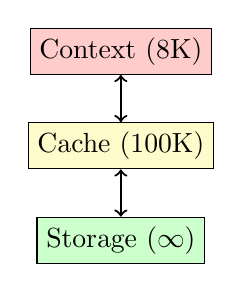
\begin{tikzpicture}[scale=0.6]
				\node[rectangle, draw, fill=red!20] (ctx) at (0,2) {Context (8K)};
				\node[rectangle, draw, fill=yellow!20] (cache) at (0,0) {Cache (100K)};
				\node[rectangle, draw, fill=green!20] (disk) at (0,-2) {Storage ($\infty$)};
				
				\draw[<->, thick] (ctx) -- (cache);
				\draw[<->, thick] (cache) -- (disk);
			\end{tikzpicture}
		\end{center}
		
		\textbf{Applications:}
		\begin{itemize}
			\item Document analysis beyond context
			\item Multi-session conversations
			\item Persistent agent memory
		\end{itemize}
	\end{columns}
	
	\vspace{0.3cm}
	\small
	Packer et al., October 2023
\end{frame}

\begin{frame}{Toolformer: Self-Supervised Tool Learning}
	\textbf{Core Innovation:} LLMs teach themselves when and how to use tools
	
	\begin{columns}
		\column{0.5\textwidth}
		\begin{block}{API Call Format}
			\footnotesize
			\texttt{The weather is <API>}\\
			\texttt{weather("New York")}\\
			\texttt{</API> 72°F today}
		\end{block}
		
		\textbf{Training Process:}
		\begin{itemize}
			\item[1.] Sample API calls positions
			\item[2.] Execute and evaluate utility
			\item[3.] Fine-tune on useful calls
		\end{itemize}
		
		\column{0.5\textwidth}
		\textbf{Tools Integrated:}
		\begin{itemize}
			\item Calculator
			\item QA System
			\item Search Engines
			\item Translation
			\item Calendar
		\end{itemize}
		
		\textbf{Results:}
		\begin{itemize}
			\item {\color{highlight}Zero-shot} improvements across tasks
			\item Maintains language generation ability
			\item Self-supervised learning approach
		\end{itemize}
	\end{columns}
	
	\vspace{0.3cm}
	\small
	Schick et al., Meta AI, February 2023
\end{frame}

\begin{frame}{WebGPT: Browser-Assisted QA}
	\begin{columns}
		\column{0.6\textwidth}
		\textbf{First large-scale web-browsing LLM}
		
		\begin{itemize}
			\item Text-based browser environment
			\item Imitation learning from humans
			\item Reference-backed answers
		\end{itemize}
		
		\begin{block}{Browser Actions}
			\small
			\begin{itemize}
				\item \texttt{search(query)}
				\item \texttt{click(link)}
				\item \texttt{quote(text)}
				\item \texttt{scroll()}
				\item \texttt{back()}
			\end{itemize}
		\end{block}
		
		\column{0.4\textwidth}
		\textbf{Training Data:}
		\begin{itemize}
			\item 6K human demonstrations
			\item 20K preference comparisons
			\item RLHF for alignment
		\end{itemize}
		
		\textbf{Performance:}
		\begin{itemize}
			\item {\color{highlight}56\%} preferred over humans
			\item {\color{highlight}69\%} vs Reddit answers
			\item Factual answers with citations
		\end{itemize}
	\end{columns}
	
	\vspace{0.3cm}
	\small
	Nakano et al., OpenAI, December 2021
\end{frame}

\begin{frame}{Comparative Analysis}
	\begin{center}
		\small
		\begin{tabular}{|l|c|c|c|c|}
			\hline
			\textbf{Method} & \textbf{Memory} & \textbf{Tools} & \textbf{Training} & \textbf{Key Innovation} \\
			\hline
			ReAct & Limited & External & Few-shot & Reasoning traces \\
			MemGPT & {\color{highlight}Unlimited} & Basic & N/A & Virtual memory \\
			Toolformer & Limited & {\color{highlight}5 types} & Self-supervised & Auto tool learning \\
			WebGPT & Limited & Browser & {\color{highlight}RLHF} & Web grounding \\
			AutoGPT & Short+Long & Extensible & None & {\color{highlight}Self-prompting} \\
			\hline
		\end{tabular}
	\end{center}
	
	\vspace{0.5cm}
	
	\textbf{Current Trends:}
	\begin{columns}
		\column{0.5\textwidth}
		\begin{itemize}
			\item Multi-agent systems
			\item Continuous learning
			\item Tool creation
		\end{itemize}
		
		\column{0.5\textwidth}
		\begin{itemize}
			\item Code generation agents
			\item Embodied agents
			\item Scientific discovery
		\end{itemize}
	\end{columns}
	
	\vspace{0.3cm}
	\textbf{Open Challenges:} Reliability, safety, evaluation metrics, cost
\end{frame}

% ==========================
% Section 4: Case Study - Claude Code (15 pages)
% ==========================
\section{Case Study: Claude Code}

\begin{frame}
	\begin{center}
		\Large
		\textbf{Case Study: Claude Code}
	\end{center}
\end{frame}

\begin{frame}[fragile]{Claude Code: Introduction}
	\begin{columns}
		\column{0.6\textwidth}
		\textbf{What is Claude Code?}
		\begin{itemize}
			\item {\color{highlight}Anthropic's official CLI} for Claude, an AI-powered coding assistant
			\item Release in Feb 2025
			\item Source code is available at: https://github.com/anthropics/claude-code with obfuscated code
		\end{itemize}
		
		\textbf{Models Used:}
		\begin{itemize}
			\item Haiku 3.5 (simple tasks, high throughput)
			\item Sonnet 4 (main agent) 
			\item Opus 4.1 (complex tasks)
		\end{itemize}
	\end{columns}
\end{frame}

\begin{frame}{Architecture: Multi-Agent System}
	\begin{center}
		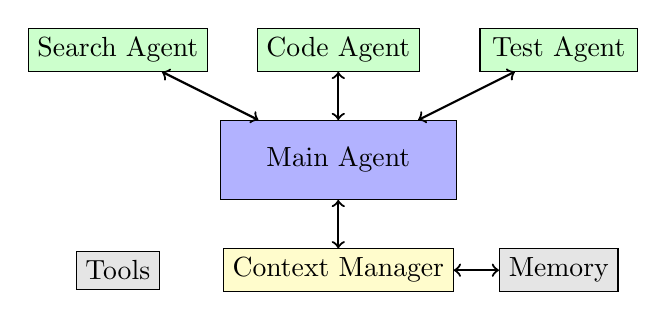
\begin{tikzpicture}[scale=0.7]
			% Main Agent
			\node[rectangle, draw, fill=blue!30, minimum width=3cm, minimum height=1cm] (main) at (0,0) {Main Agent};
			
			% Sub-agents
			\node[rectangle, draw, fill=green!20, minimum width=2cm] (search) at (-4,2) {Search Agent};
			\node[rectangle, draw, fill=green!20, minimum width=2cm] (code) at (0,2) {Code Agent};
			\node[rectangle, draw, fill=green!20, minimum width=2cm] (test) at (4,2) {Test Agent};
			
			% Context Manager
			\node[rectangle, draw, fill=yellow!20, minimum width=2cm] (context) at (0,-2) {Context Manager};
			
			% Tools
			\node[rectangle, draw, fill=gray!20] (tools) at (-4,-2) {Tools};
			\node[rectangle, draw, fill=gray!20] (memory) at (4,-2) {Memory};
			
			% Connections
			\draw[<->, thick] (main) -- (search);
			\draw[<->, thick] (main) -- (code);
			\draw[<->, thick] (main) -- (test);
			\draw[<->, thick] (main) -- (context);
			\draw[<->, thick] (context) -- (memory);
		\end{tikzpicture}
	\end{center}
	
	\begin{itemize}
		\item {\color{highlight}\textbf{Main Agent}}: Orchestrates overall task
		\item {\color{highlight}\textbf{Sub-agents}}: Handle specific subtasks in isolation
		\item {\color{highlight}\textbf{Context Manager}}: Optimizes token usage
	\end{itemize}
\end{frame}


\begin{frame}{Reverse Engineering: System Prompts}
	\textbf{Key System Prompt Elements:}
	
	\begin{block}{Core Instructions}
		\footnotesize
		\begin{itemize}
			\item "You are Claude Code, Anthropic's official CLI for Claude"
			\item "Be concise, direct, and to the point"
			\item "Minimize output tokens while maintaining quality"
			\item "Use tools to complete tasks, not for communication"
		\end{itemize}
	\end{block}
	
	\textbf{Behavioral Guidelines:}
	\begin{columns}
		\column{0.5\textwidth}
		\begin{itemize}
			\item {\color{highlight}Proactive}: Use TODO lists
			\item {\color{highlight}Defensive}: Follow conventions
			\item {\color{highlight}Efficient}: Batch operations
		\end{itemize}
		
		\column{0.5\textwidth}
		\begin{itemize}
			\item {\color{highlight}Safe}: Never commit without asking
			\item {\color{highlight}Clear}: Explain complex commands
			\item {\color{highlight}Adaptive}: Learn from context
		\end{itemize}
	\end{columns}
	
	\small
	Source: github.com/Yuyz0112/claude-code-reverse
\end{frame}

\begin{frame}{Agentic Workflow}
	\begin{itemize}
		\item[1.] {\color{highlight}\textbf{Quota Check}} (Haiku 3.5)
		\begin{itemize}
			\item Lightweight API verification
			\item Context initialization
		\end{itemize}
		
		\item[2.] {\color{highlight}\textbf{Task Analysis}} (Main Agent)
		\begin{itemize}
			\item Parse user request
			\item Create TODO list
			\item Plan execution strategy
		\end{itemize}
		
		\item[3.] {\color{highlight}\textbf{Execution Loop}}
		\begin{itemize}
			\item Execute tools in parallel when possible
			\item Update TODO status
			\item Handle errors and retry
		\end{itemize}
		
		\item[4.] {\color{highlight}\textbf{Context Compaction}}
		\begin{itemize}
			\item Isolate "dirty context" in sub-agents
			\item Return only essential results
			\item Maintain conversation history
		\end{itemize}
	\end{itemize}
\end{frame}

\begin{frame}[fragile]{TODO List: How It Works}
	\textbf{Core Mechanism:}
	\begin{itemize}
		\item {\color{highlight}\textbf{Proactive Creation}}: Agent creates TODO list for complex tasks (3+ steps)
		\item {\color{highlight}\textbf{Real-time Updates}}: Status changes as work progresses
		\item {\color{highlight}\textbf{Atomic Operations}}: Each task marked complete immediately upon finish
	\end{itemize}
	
	\begin{columns}
		\column{0.5\textwidth}
		\begin{block}{JSON Structure}
			\footnotesize
			\begin{lstlisting}[basicstyle=\tiny]
{
  "todos": [
    {
      "content": "Fix authentication bug",
      "activeForm": "Fixing authentication bug", 
      "status": "in_progress"
    },
    {
      "content": "Run tests",
      "activeForm": "Running tests",
      "status": "pending"  
    }
  ]
}
			\end{lstlisting}
		\end{block}
		
		\column{0.5\textwidth}
		\textbf{Workflow:}
		\begin{itemize}
			\item[1.] User requests complex task
			\item[2.] Agent creates TODO list
			\item[3.] Exactly ONE task "in\_progress" 
			\item[4.] Complete → mark done → start next
			\item[5.] Continue until all complete
		\end{itemize}
		
		\textbf{Key Rules:}
		\begin{itemize}
			\item Never batch completions
			\item One active task only
			\item Clear, actionable items
		\end{itemize}
	\end{columns}
\end{frame}

\begin{frame}{TODO List: Dynamic Task Management}
	\begin{columns}
		\column{0.5\textwidth}
		\includegraphics[width=\textwidth]{fig/TODO1.jpg}
		
		\column{0.5\textwidth}
		\textbf{Implementation:}
		\begin{itemize}
			\item Stored in \texttt{\~{}/.claude/todos/}
			\item JSON format
			\item Three states:
			\begin{itemize}
				\item \texttt{pending}
				\item \texttt{in\_progress}
				\item \texttt{completed}
			\end{itemize}
		\end{itemize}
		
		\textbf{Benefits:}
		\begin{itemize}
			\item User visibility
			\item Progress tracking
			\item Task decomposition
			\item Error recovery
		\end{itemize}
	\end{columns}
\end{frame}

\begin{frame}{TODO List: Real Example}
	\includegraphics[width=0.8\textwidth]{fig/TODO2.jpg}
	
	\begin{itemize}
		\item {\color{highlight}Automatic creation} when task complexity detected
		\item {\color{highlight}Real-time updates} as work progresses
		\item {\color{highlight}Hierarchical} task breakdown
	\end{itemize}
\end{frame}

\begin{frame}[fragile]{Test Case: Scientific Computing (99\%)}
	\textbf{Task:} Understand complex numerical package: GPAW (electronic structure calculation) 300K+ lines of code
	
	\begin{block}{Claude Code Performance}
		\begin{itemize}
			\item $\checkmark$ Trace functions and classes without Go to Definition
			\item $\checkmark$ Connect mathematical derivations and code implementation
			\item $\checkmark$ Analyze the implementation efficiency
		\end{itemize}
	\end{block}
	
	\begin{lstlisting}[language=python, basicstyle=\tiny]
# Claude correctly identified spectral method
def spectral_solver(u, dt, nu):
    """Solve 2D Navier-Stokes using FFT"""
    u_hat = fft2(u)
    # Claude: "Using semi-implicit time stepping 
    # for stability with explicit nonlinear terms"
    nonlinear = compute_nonlinear(u)
    u_hat = (u_hat + dt * fft2(nonlinear)) / (1 + nu * dt * k2)
    return ifft2(u_hat)
	\end{lstlisting}
\end{frame}

\begin{frame}[fragile]{Test Case: Environment Setup (99\%)}
	\textbf{Task:} Modify Docker configuration for ML pipeline
	
	\begin{columns}
		\column{0.5\textwidth}
		\begin{block}{Original Dockerfile}
			\footnotesize
			\begin{lstlisting}[basicstyle=\tiny]
FROM python:3.8
RUN pip install numpy
CMD ["python", "app.py"]
			\end{lstlisting}
		\end{block}
		
		\column{0.5\textwidth}
		\begin{block}{Claude's Modification}
			\footnotesize
			\begin{lstlisting}[basicstyle=\tiny]
FROM python:3.8-slim
WORKDIR /app
COPY requirements.txt .
RUN pip install --no-cache-dir -r requirements.txt
COPY . .
CMD ["python", "-u", "app.py"]
			\end{lstlisting}
		\end{block}
	\end{columns}
	
	\textbf{Improvements Made:}
	\begin{itemize}
		\item Used slim image (reduced size)
		\item Added proper layer caching
		\item Implemented best practices
		\item Added unbuffered output
	\end{itemize}
\end{frame}

\begin{frame}[fragile]{Test Case: Unit Testing}
	\textbf{Task:} Write comprehensive unit tests
	
	\begin{lstlisting}[language=python, basicstyle=\tiny]
# Claude generated test with edge cases
def test_matrix_operations():
    """Test matrix multiplication with various inputs"""
    # Test normal case
    assert multiply([[1,2],[3,4]], [[5,6],[7,8]]) == [[19,22],[43,50]]
    
    # Test identity
    I = [[1,0],[0,1]]
    A = [[1,2],[3,4]]
    assert multiply(A, I) == A
    
    # Test zero matrix
    Z = [[0,0],[0,0]]
    assert multiply(A, Z) == Z
    
    # Test dimension mismatch
    with pytest.raises(ValueError):
        multiply([[1,2]], [[1],[2],[3]])
	\end{lstlisting}
	
	{\color{highlight}Key: Clear interface + complete instructions = High success}
\end{frame}

\begin{frame}{Test Case: Debug NS Solver (40\%)}
	\textbf{Task:} Debug hand-written spectral solver for 2D Navier-Stokes
	
	\textbf{Challenges Encountered:}
	\begin{itemize}
		\item {\color{red}$\times$} Complex aliasing errors
		\item {\color{red}$\times$} Numerical stability issues  
		\item {\color{orange}$\triangle$} Identified problem areas
		\item {\color{red}$\times$} Could not fix without domain expertise
	\end{itemize}
	
	\textbf{Lesson:} Claude Code struggles with:
	\begin{itemize}
		\item Deep domain-specific knowledge
		\item Numerical analysis subtleties
		\item Complex debugging requiring intuition
	\end{itemize}
\end{frame}

\begin{frame}{Test Case: Hydra Configuration (20\%)}
	\textbf{Task:} Set up Hydra for multi-run experiments
	
	\textbf{Issues:}
	\begin{itemize}
		\item {\color{red}$\times$} Misunderstood Hydra's configuration structure
		\item {\color{red}$\times$} Generated incorrect sweep syntax
		\item {\color{red}$\times$} Failed to handle composition properly
	\end{itemize}
	
	\textbf{Root Cause:}
	\begin{itemize}
		\item Limited training data on Hydra
		\item Complex configuration inheritance
		\item Framework-specific patterns
	\end{itemize}
\end{frame}

\begin{frame}{Claude Code as a Tool for Humans}
	\textbf{Key Insight:} {\color{highlight}Dramatically lowers barriers} for many tasks
	
	\begin{columns}
		\column{0.5\textwidth}
		\textbf{Before Claude Code:}
		\begin{itemize}
			\item Hours reading documentation
			\item Manual environment setup
			\item Trial-and-error debugging
			\item Context switching overhead
		\end{itemize}
		
		\column{0.5\textwidth}
		\textbf{With Claude Code:}
		\begin{itemize}
			\item Instant codebase understanding
			\item Automated setup scripts
			\item Guided exploration
			\item Maintained context
		\end{itemize}
	\end{columns}
	
	\vspace{0.5cm}
	
	\begin{block}{Best Use Cases}
		\begin{itemize}
			\item {\color{highlight}Learning new repositories}: Navigate unfamiliar codebases
			\item {\color{highlight}Environment setup}: Docker, dependencies, configuration
			\item {\color{highlight}Boilerplate generation}: Tests, documentation, CI/CD
			\item {\color{highlight}Refactoring}: Systematic code improvements
		\end{itemize}
	\end{block}
\end{frame}

\begin{frame}{Lessons from Claude Code}
	\textbf{Architectural Insights:}
	\begin{itemize}
		\item {\color{highlight}Multi-agent} design scales better than monolithic
		\item {\color{highlight}Context management} is crucial for long tasks
		\item {\color{highlight}TODO lists} provide structure and visibility
	\end{itemize}
	
	\textbf{Practical Implications:}
	\begin{itemize}
		\item Works best with {\color{highlight}clear specifications}
		\item Excels at {\color{highlight}well-defined tasks}
		\item Struggles with {\color{highlight}domain-specific expertise}
	\end{itemize}
	
	\textbf{Future Directions:}
	\begin{itemize}
		\item Better memory systems (MemGPT-style)
		\item Improved error recovery
		\item Domain-specific fine-tuning
		\item Multi-modal capabilities (diagrams, UI)
	\end{itemize}
\end{frame}

\begin{frame}{Performance Summary}
	\begin{center}
		\begin{tabular}{|l|c|p{5cm}|}
			\hline
			\textbf{Task Type} & \textbf{Score} & \textbf{Key Factors} \\
			\hline
			Code Reading & {\color{green}99\%} & Pattern recognition, documentation \\
			Environment Setup & {\color{green}99\%} & Standard practices, clear goals \\
			Unit Testing & {\color{green}95\%} & Clear interfaces, specifications \\
			Complex Debug & {\color{orange}40\%} & Needs domain expertise \\
			Framework Config & {\color{red}20\%} & Limited training data \\
			Novel Algorithms & {\color{red}N/A} & Beyond current capabilities \\
			\hline
		\end{tabular}
	\end{center}
	
	\vspace{0.5cm}
	
	\textbf{Key Takeaway:}
	\begin{center}
		\large
		{\color{highlight}Claude Code is a powerful amplifier for human developers,}\\
		{\color{highlight}not a replacement for domain expertise}
	\end{center}
\end{frame}


\begin{frame}{}
	\begin{center}
		\Huge Thank You!
		
		\vspace{1cm}
		
		\Large Questions?
	\end{center}
\end{frame}

\end{document}